\documentclass[11pt,a4paper]{article}
\usepackage[utf8]{inputenc}
\usepackage[portuguese]{babel}
\usepackage[T1]{fontenc}
\usepackage{amsmath}
\usepackage{amsfonts}
\usepackage{amssymb}
\usepackage{graphicx}
\author{Eduardo Adame}
\title{Primeiro Documento Curso \LaTeX}
\begin{document}
\maketitle
\newpage
\tableofcontents
\newpage
\section{\textsc{Primeiros passos}}

\subsection{Texto Simples}
\label{ss:ts}
Hoje é um dia feliz, estou começando no \LaTeX .\\


\subsection{Tamanhos e Tipos de Textos}
% Utilizar \textbf{} (ou derivados) com texto dentro das chaves para alterar o tipo. É possivel utilizar mais que um.

% Utilizar \Large dentro das chaves junto ao texto para alterar tamanho da linha.
{\Large Eu \textbf{gosto} de} \textbf{\textit{comer}} \textsc{mamão}.

\section{Ambientes}
Itens que eu gosto de comprar na padaria Camila
\begin{enumerate}
\item Salgado de 1 Real
\item Suco de Maracujá
\item Coquinha KS
\item Pão de Queijo
\item Misto 
\begin{enumerate}
\item Quente
\item Frio
\end{enumerate}
\item Esfirra 
\end{enumerate}

\begin{itemize}
\item[O MELHOR] Salgado de 1 Real
\item Suco de Maracujá
\item Coquinha KS
\item Pão de Queijo
\item Misto Quente
\item Esfirra
\item Kibe 
\end{itemize}

\newpage
\section{Notas de Rodapé}

Stardust: Gente que voa\footnote{SANTOS, Paulo. Itajubá, 2019}.\\
SPACEX: Especialista em ser sexy\footnote{REIS, Marcelo. Itajubá, 2019}.

\section{Texto Matemático}

% EM LINHA
Essa é uma fração: $\dfrac{\mu^2 - \rho_2}{\nabla - 4 \cdot 25} \leftrightharpoons \theta_b^a$
% DESTACADO
$$\dfrac{\mu^2 - \rho_2}{\nabla - 4 \cdot 25} \leftrightharpoons \theta_b^a$$
% CRIA NUMERAÇÃO
\begin{equation}
\dfrac{\mu^2 - \rho_2}{\nabla - 4 \cdot 25} \leftrightharpoons \theta_b^a 10
% REFERENCIA
\label{eq:doida}
\end{equation}

Olhando para a equação \eqref{eq:doida}, você vê que eu não sei nada. Lembra da seção \ref{ss:ts}?

\newpage
\section{Adicionando Imagens}

OLHE ESTA IMAGEM
\begin{figure}[!h]
\centering
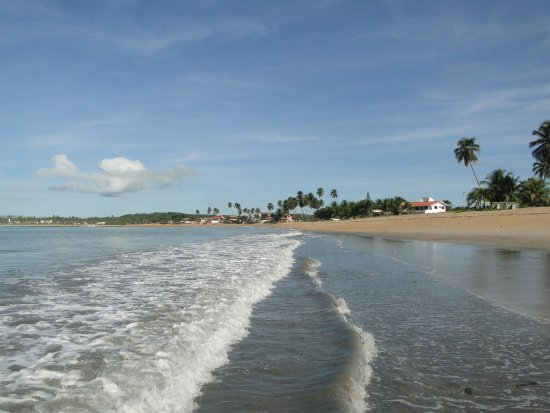
\includegraphics[width=.8\textwidth]{1.jpg}
\caption{Figura Inexistente}
\end{figure}
\end{document}


















